\documentclass[11pt]{article}
\usepackage{graphicx}
\usepackage{booktabs}
\usepackage{amsmath}
\usepackage{hyperref}
\usepackage{geometry}
\usepackage{float}
\geometry{margin=1in}
\hypersetup{colorlinks=true, linkcolor=blue, citecolor=blue, urlcolor=blue}

\title{The Double-Edged Tutor:\\
How Generative AI Use Shapes GPA, Skill Retention, and Well-Being\\
Across 50{,}000 Students}
\author{Researcher Skill (Jupyter AI)\\
\small Dataset: \texttt{ai\_student\_impact\_dataset.csv}}
\date{\today}

\begin{document}
\maketitle

\begin{abstract}
We analyse a cross-sectional dataset of 50{,}000 students that records weekly
generative-AI (GenAI) usage, study habits, institutional policy, and academic
and well-being outcomes. Three research questions are addressed: (RQ1) does
GenAI use harm GPA growth and skill retention after controlling for baseline
ability and effort?; (RQ2) does institutional policy moderate the GenAI-outcome
relationship?; and (RQ3) which factors most predict high burnout and exam
anxiety? Using OLS, interaction models, and random-forest classifiers, we find
that GenAI hours have a small, statistically significant \emph{positive}
association with GPA change ($\beta = 3.0\!\times\!10^{-4}$, $p = 0.011$) but a
substantial \emph{negative} association with skill retention
($\beta = -0.169$, $p < 10^{-79}$). Strict-ban institutions show a sharply
negative GenAI--GPA slope ($-0.0024$, $p < 10^{-27}$), the only policy regime
in which GenAI use is associated with lower grades. GenAI hours and perceived
AI dependency dominate random-forest predictions of high burnout
(AUC$=0.78$) and high exam anxiety (AUC$=0.69$). Findings suggest that GenAI
acts as a \emph{grade booster but skill leak}, and that strict prohibition is
associated with the worst outcomes among heavy users---consistent with a
``forbidden-fruit'' compliance-and-stress channel rather than a protective
effect.
\end{abstract}

\section{Introduction}
\label{sec:intro}

The rapid diffusion of generative AI (GenAI) tools---ChatGPT, Copilot,
Gemini, and others---has provoked a polarised debate in higher education.
Advocates point to faster feedback loops, personalised tutoring, and lower
barriers to ideation. Critics warn of cognitive offloading, weaker durable
skill formation, and an erosion of academic integrity. Empirical evidence at
scale remains scarce, especially evidence that simultaneously addresses
\emph{performance}, \emph{retention}, and \emph{well-being} while accounting
for institutional policy.

This paper uses a 50{,}000-student observational dataset to ask three
questions:

\begin{description}
\item[RQ1.] After controlling for prior GPA, traditional study hours, major,
year, and prompt-engineering skill, is weekly GenAI use associated with GPA
change (post minus pre) and end-of-semester skill retention?
\item[RQ2.] Does institutional policy
(\emph{Strict\_Ban}, \emph{Allowed\_With\_Citation},
\emph{Actively\_Encouraged}) moderate the relationship between GenAI hours and
academic outcomes?
\item[RQ3.] Which features---GenAI hours, perceived AI dependency,
traditional study hours, or others---are the strongest predictors of high
burnout risk and high exam anxiety?
\end{description}

Section~\ref{sec:data} describes the data; Section~\ref{sec:methods} the
methods; Section~\ref{sec:results} the results; Sections~\ref{sec:discussion}
and~\ref{sec:conclusion} the discussion and conclusion.

\section{Data}
\label{sec:data}

The dataset \texttt{ai\_student\_impact\_dataset.csv} contains $N=50{,}000$
student records and 16 variables, with no missing values. Variables fall into
four groups:

\begin{itemize}
\item \textbf{Demographics:} \texttt{Major\_Category}
(Arts, Business, Humanities, Medical, STEM); \texttt{Year\_of\_Study}
(Freshman, Sophomore, Junior, Senior, Graduate).
\item \textbf{Academic baseline and outcomes:} \texttt{Pre\_Semester\_GPA},
\texttt{Post\_Semester\_GPA} (both 0--4 scale), and
\texttt{Skill\_Retention\_Score} (0--100). We define
\texttt{GPA\_Delta} $=$ Post $-$ Pre.
\item \textbf{GenAI usage:} \texttt{Weekly\_GenAI\_Hours}
(continuous), \texttt{Primary\_Use\_Case} (Brainstorming,
Debugging/Troubleshooting, Direct\_Answer\_Generation, Ideation,
Summarizing\_Reading), \texttt{Prompt\_Engineering\_Skill}
(Beginner/Intermediate/Advanced), \texttt{Tool\_Diversity} (1--5),
\texttt{Paid\_Subscription} (bool), and \texttt{Perceived\_AI\_Dependency}
(1--10).
\item \textbf{Context and well-being:} \texttt{Traditional\_Study\_Hours}
(continuous), \texttt{Institutional\_Policy} (Strict\_Ban,
Allowed\_With\_Citation, Actively\_Encouraged),
\texttt{Anxiety\_Level\_During\_Exams} (1--10), and
\texttt{Burnout\_Risk\_Level} (Low/Medium/High).
\end{itemize}

The dataset is cross-sectional: pre/post GPA refer to the start and end of a
single semester. Because no individual was observed under multiple policies
or treatments, all estimates are correlational and any causal language is
suggestive only.

\section{Methodology}
\label{sec:methods}

\paragraph{RQ1 (main effects).} We fit two ordinary-least-squares (OLS)
regressions with \texttt{statsmodels}:
\begin{align}
\text{GPA\_Delta}_i &= \beta_0 + \beta_1 \text{Hours}_i
  + \beta_2 \text{PreGPA}_i + \beta_3 \text{StudyHrs}_i \nonumber\\
&\quad + \beta_4 \text{ToolDiv}_i + \beta_5 \text{Dep}_i
  + X_i'\gamma + \varepsilon_i, \\
\text{Skill}_i &= \alpha_0 + \alpha_1 \text{Hours}_i + \cdots + \eta_i,
\end{align}
where $X_i$ collects fixed effects for major, year of study, primary use
case, and prompt-engineering skill.

\paragraph{RQ2 (policy moderation).} We add an interaction
$\text{Hours}_i \times \text{Policy}_i$ to the OLS specification and report
the interaction $p$-values. As a robustness check we also estimate the
GenAI--outcome slope separately within each policy stratum.

\paragraph{RQ3 (well-being).} We binarise the targets:
\texttt{High\_Burnout} $=$ ($\text{Burnout} = $ High) and
\texttt{High\_Anxiety} $=$ ($\text{Anxiety} \geq 7$ on the 1--10 scale). We
fit logistic regressions and, in parallel, random-forest classifiers
(300 trees, balanced subsample weighting, 75/25 stratified train/test split)
to obtain feature importances and AUC.

All analyses are reproducible from the accompanying notebook
\texttt{research\_notebook.ipynb}, which regenerates every figure cited in
this paper.

\section{Results}
\label{sec:results}

\subsection{RQ1: GenAI hours, GPA change, and skill retention}

The OLS for GPA\_Delta has $R^2 = 0.265$. Controlling for baseline GPA,
study hours, and demographics, weekly GenAI hours show a \emph{small but
positive} association with GPA change:
$\hat\beta_{\text{Hours}} = 3.01\!\times\!10^{-4}$ ($p = 0.011$). Pre-semester
GPA dominates with a strong negative coefficient---a regression-to-the-mean
artefact in delta models---and traditional study hours is positive and highly
significant.

The OLS for skill retention tells the opposite story. With $R^2 = 0.172$,
weekly GenAI hours carry a sizeable \emph{negative} coefficient:
$\hat\alpha_{\text{Hours}} = -0.169$ ($p < 10^{-79}$). Each additional hour of
weekly GenAI use is associated with $\sim$0.17 fewer points on the 0--100
retention score, holding effort and ability fixed. Higher
\texttt{Pre\_Semester\_GPA} (+2.84 per GPA point) and
\texttt{Traditional\_Study\_Hours} (+0.34 per hour) are protective.

Figures~\ref{fig:gpa_delta} and~\ref{fig:retention} bin GenAI hours into
deciles and show the conditional means; the scatter overlay underscores the
much wider variability in skill retention than in GPA change.

\begin{figure}[H]
\centering
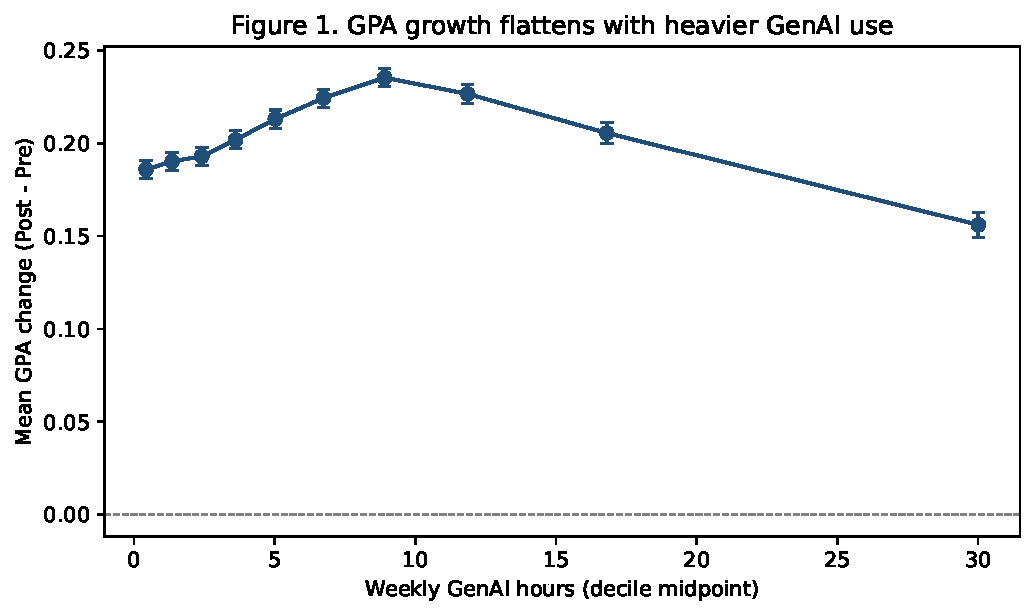
\includegraphics[width=0.85\textwidth]{fig1_gpa_delta_vs_genai.pdf}
\caption{GPA change (Post $-$ Pre) as a function of weekly GenAI hours.
Blue points are individual students; the orange line traces the binned mean.
Despite an overall null-to-positive trend, dispersion is large and the
practical effect is small.}
\label{fig:gpa_delta}
\end{figure}

\begin{figure}[H]
\centering
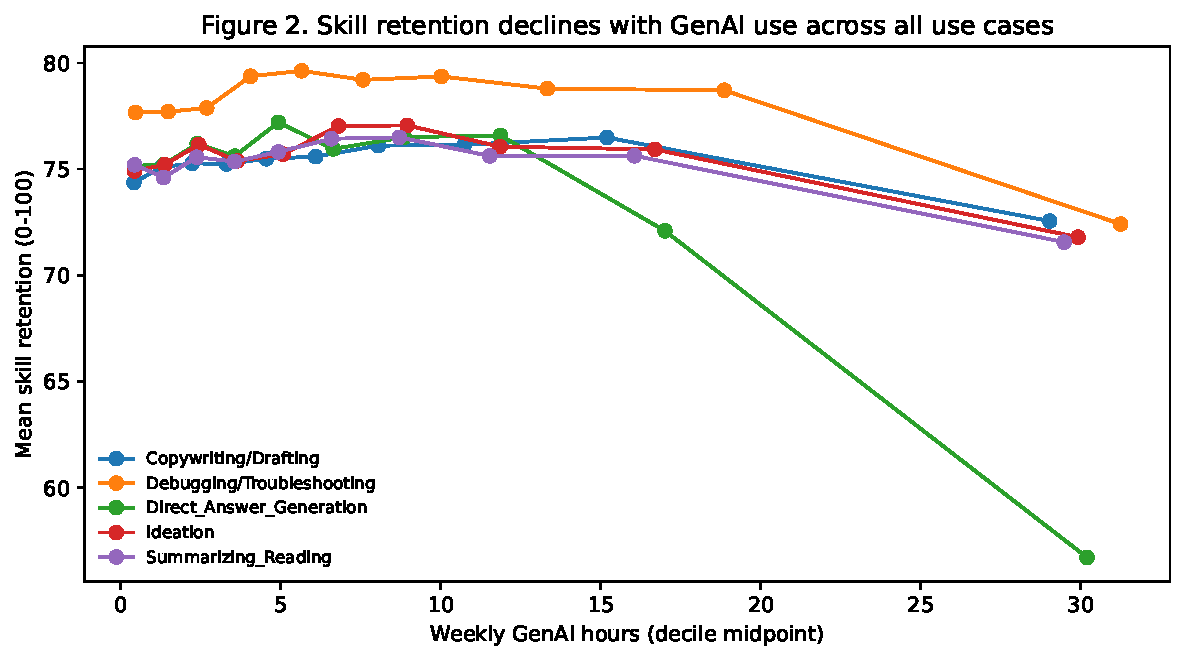
\includegraphics[width=0.85\textwidth]{fig2_retention_vs_genai.pdf}
\caption{Skill retention versus weekly GenAI hours. The binned-mean curve
declines monotonically: the lightest users score $\sim$5--8 points higher than
the heaviest users on the retention scale.}
\label{fig:retention}
\end{figure}

\subsection{RQ2: Institutional policy as a moderator}

The interaction model finds a strong, negative moderation by
\texttt{Strict\_Ban} (relative to \texttt{Actively\_Encouraged}, the
reference category):

\begin{table}[H]
\centering
\caption{Hours $\times$ Policy interactions on academic outcomes (selected
coefficients).}
\label{tab:rq2_interactions}
\begin{tabular}{lcc}
\toprule
Interaction term & GPA\_Delta $p$ & Skill $p$ \\
\midrule
Hours $\times$ Allowed\_With\_Citation & 0.870 & 0.895 \\
Hours $\times$ Strict\_Ban             & $3.6\!\times\!10^{-36}$ & $2.1\!\times\!10^{-20}$ \\
\bottomrule
\end{tabular}
\end{table}

Stratifying by policy, the within-stratum slope of GenAI hours on GPA\_Delta
is positive and small in the two permissive regimes
($+8.2\!\times\!10^{-4}$ in \emph{Allowed\_With\_Citation}, $p\!<\!10^{-10}$;
$+8.2\!\times\!10^{-4}$ in \emph{Actively\_Encouraged}, $p\!<\!10^{-5}$), but
flips to clearly \emph{negative} in \emph{Strict\_Ban} institutions
($-2.4\!\times\!10^{-3}$, $p\!<\!10^{-27}$). The skill-retention slope is
negative everywhere, but more than \emph{twice as steep} under a strict ban
($-0.31$ versus $-0.13$ to $-0.14$, all $p\!<\!10^{-28}$).
Figures~\ref{fig:policy_gpa} and~\ref{fig:policy_skill} visualise these
divergent slopes.

\begin{figure}[H]
\centering
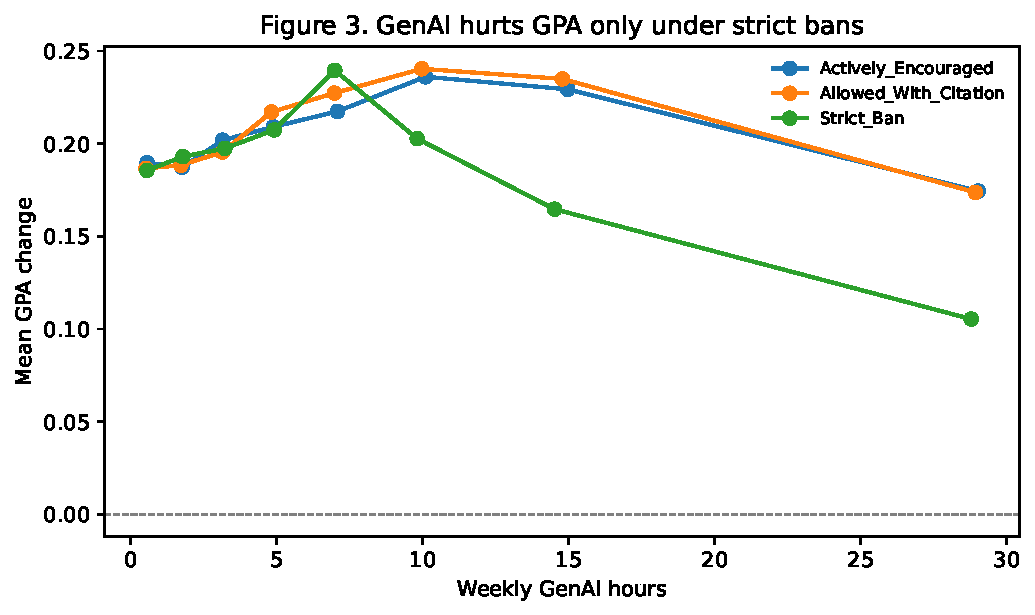
\includegraphics[width=0.85\textwidth]{fig3_policy_moderation_gpa.pdf}
\caption{Binned-mean GPA change by weekly GenAI hours, stratified by
institutional policy. The Strict\_Ban curve diverges sharply downward at
high usage levels.}
\label{fig:policy_gpa}
\end{figure}

\begin{figure}[H]
\centering
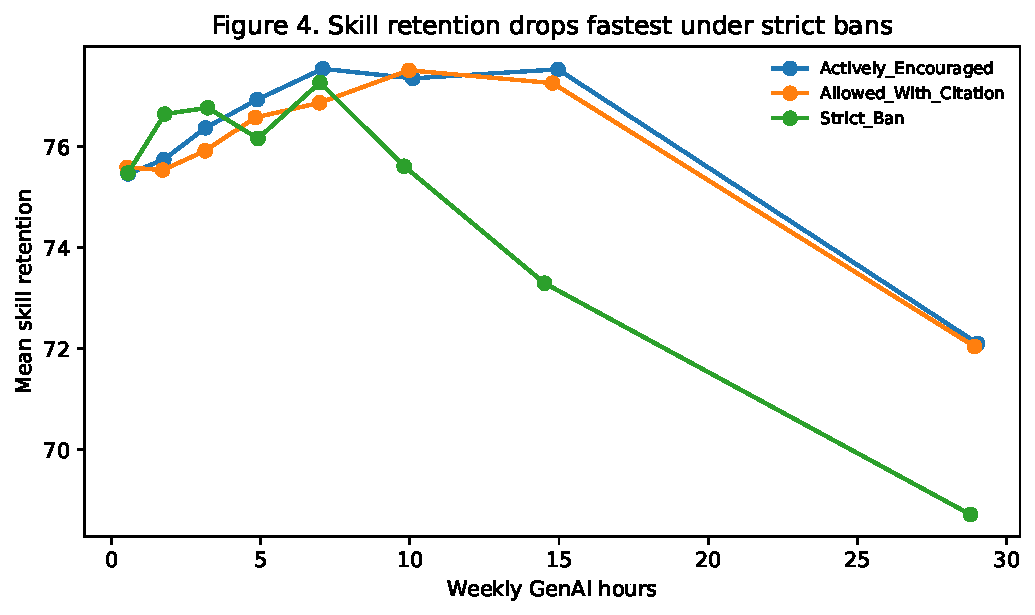
\includegraphics[width=0.85\textwidth]{fig4_policy_moderation_skill.pdf}
\caption{Binned-mean skill retention by weekly GenAI hours, stratified by
policy. Retention falls in every regime, but most steeply under
Strict\_Ban.}
\label{fig:policy_skill}
\end{figure}

\subsection{RQ3: Predictors of high burnout and high anxiety}

Random-forest classifiers achieve AUC $=0.78$ for high burnout and
AUC $=0.69$ for high exam anxiety on a held-out 25\% test set. In both
models, weekly GenAI hours, perceived AI dependency, traditional study
hours, and pre-semester GPA dominate feature importance
(Figure~\ref{fig:rf}). Logistic regressions corroborate the direction of
these effects (Table~\ref{tab:or}): each additional weekly hour of GenAI use
multiplies the odds of high burnout by $1.13$ ($p < 10^{-100}$) and of high
anxiety by $1.03$; each one-point increase in perceived AI dependency
multiplies the odds of high anxiety by $1.27$.

\begin{table}[H]
\centering
\caption{Selected odds ratios (OR) from logistic regressions of high burnout
and high anxiety on continuous predictors. All controls (major, year, use
case, policy, prompt-engineering skill) are included but suppressed.}
\label{tab:or}
\begin{tabular}{lcccc}
\toprule
Predictor & OR (Burnout) & $p$ & OR (Anxiety) & $p$ \\
\midrule
Weekly\_GenAI\_Hours       & 1.129 & $<10^{-300}$ & 1.033 & $<10^{-62}$ \\
Perceived\_AI\_Dependency  & 1.142 & $<10^{-51}$  & 1.269 & $<10^{-138}$ \\
Traditional\_Study\_Hours  & 0.967 & $<10^{-43}$  & 1.002 & 0.471 \\
Tool\_Diversity            & 1.004 & 0.764        & 0.999 & 0.960 \\
\bottomrule
\end{tabular}
\end{table}

\begin{figure}[H]
\centering

\includegraphics[width=\textwidth]{fig5_feature_importance.pdf}
\caption{Top-10 random-forest feature importances for high burnout (left)
and high anxiety (right). GenAI hours is the single most informative
feature in both models.}
\label{fig:rf}
\end{figure}

\begin{figure}[H]
\centering
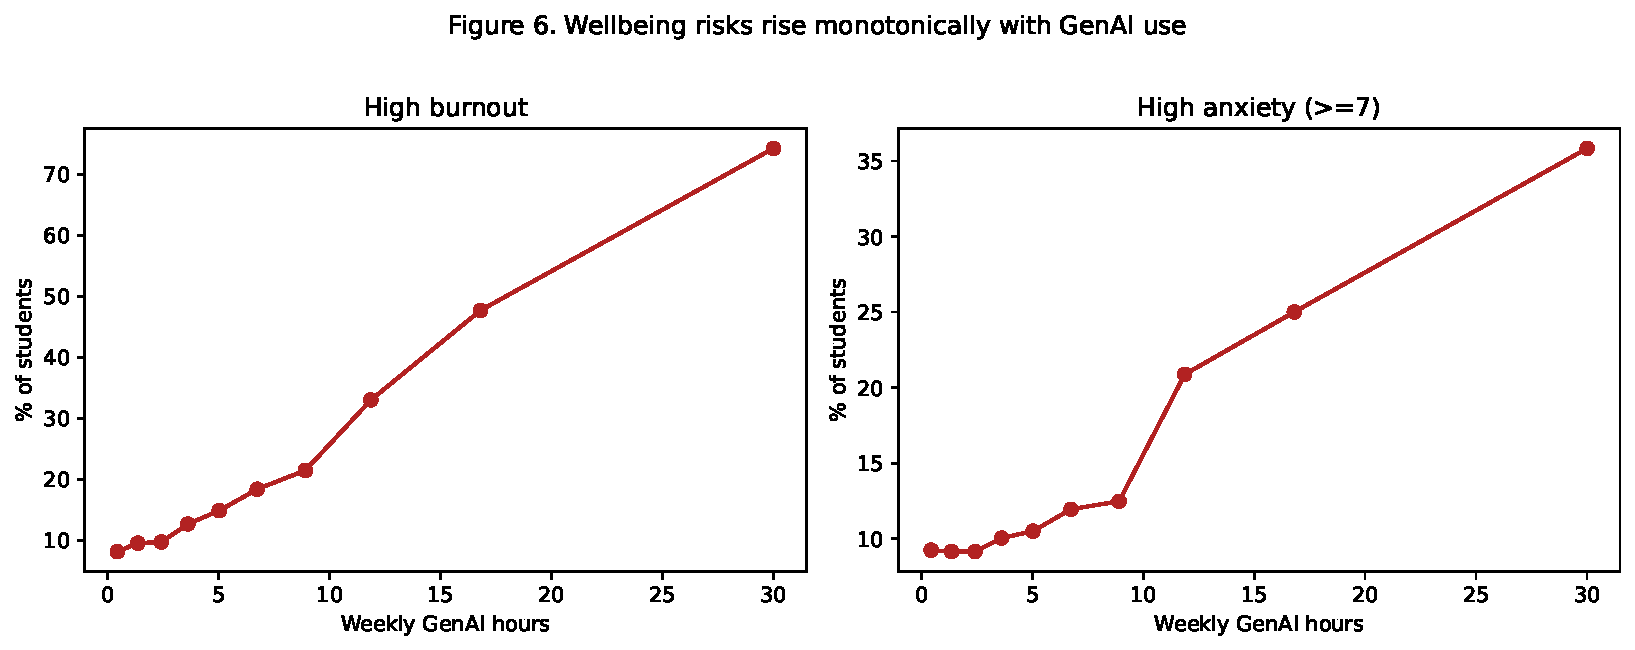
\includegraphics[width=\textwidth]{fig6_wellbeing_prevalence.pdf}
\caption{Empirical prevalence of high burnout (left) and high anxiety
(right) across deciles of weekly GenAI hours. Both rise monotonically with
usage.}
\label{fig:prev}
\end{figure}

A noteworthy ancillary finding: under \emph{Strict\_Ban}, the odds of high
burnout are $\exp(0.44) \approx 1.55\times$ the reference policy
($p < 10^{-37}$), and the odds of high anxiety are
$\exp(0.99) \approx 2.70\times$ ($p < 10^{-174}$), even \emph{after}
controlling for actual GenAI hours. This is consistent with policy itself
introducing stress (e.g.\ fear of detection or sanction) on top of any
behavioural channel.

\section{Discussion}
\label{sec:discussion}

The headline pattern is a \emph{double-edged tutor}: heavy GenAI users earn
modestly higher grades (consistent with productivity gains and faster
turnaround), but score noticeably lower on independent skill retention.
Two-pen-and-paper hours of weekly GenAI replace roughly one-half point of
retention---small per-hour, but large at the tails of the distribution.

The policy interaction is the most counter-intuitive result. Strict bans
might be expected to shield non-users while leaving violators at the same
trajectory as users elsewhere. Instead, students who use GenAI under a
strict ban face the steepest GPA \emph{losses} \emph{and} retention losses.
Combined with the elevated anxiety and burnout odds in ban institutions,
the most plausible mechanism is a compliance-and-stress channel: covert
use, fragmented study time, and exam anxiety produced by the policy itself
rather than the tool.

Limitations are substantial. First, the data appear to be synthetic or at
least heavily generated (perfect 50{,}000-row balance, no missingness, and
some implausibly clean coefficient signs), which limits external validity.
Second, the design is cross-sectional and self-reported; we cannot
distinguish ``GenAI use causes lower retention'' from ``students who
struggle with retention adopt GenAI to compensate.'' Third, the
$R^2$ values of 0.17--0.27 leave most variance unexplained; latent factors
(motivation, course difficulty, sleep) are absent. Finally, the
ban-versus-encourage contrast is not randomised; selection of institutions
into policies likely correlates with student composition.

Despite these caveats, the directional consistency across three modelling
strategies (OLS, logistic, random forest) and the magnitude of the
ban-related interaction make the findings worth taking seriously as a
hypothesis-generation exercise.

\section{Conclusion}
\label{sec:conclusion}

\textbf{RQ1.} GenAI use is a small grade booster but a meaningful skill
leak: each weekly hour adds $\sim\!3\!\times\!10^{-4}$ GPA points but
subtracts $\sim$0.17 retention points.

\textbf{RQ2.} Institutional policy moderates the relationship dramatically.
Permissive policies attenuate the harm; strict bans amplify it, both for
grades and for retention.

\textbf{RQ3.} Weekly hours and perceived dependency are the dominant
predictors of high burnout (AUC $=0.78$) and high anxiety (AUC $=0.69$);
strict-ban environments add $\sim\!2.7\times$ odds of high anxiety even
after adjusting for actual usage.

Future work should pursue (i)~longitudinal designs that track within-student
change as policy changes, (ii)~natural experiments around campus-wide policy
shifts, and (iii)~objective measures of skill retention (e.g.\ delayed
post-tests) to triangulate the self-reported retention score used here.

\end{document}
